\documentclass[12pt,a4paper]{article}
\usepackage[utf8]{inputenc}
\usepackage[T1]{fontenc}
\usepackage{fontspec}
\usepackage[polish]{babel}
\usepackage{amsmath}
\usepackage{graphicx}
\usepackage[table,xcdraw]{xcolor}
\usepackage{hhline}
% ref packages
\usepackage{nameref}
% folowing  must be in this order
\usepackage{varioref}
\usepackage{hyperref}
\usepackage{cleveref}
\usepackage{placeins}
\usepackage[margin=0.6in]{geometry}
\usepackage{appendix}
\usepackage{caption}
\usepackage{colortbl}
\usepackage{physics}
\usepackage{a4wide}
\usepackage{float}
\usepackage{datetime}
\usepackage{makeidx}

\title{Termodynamika R 2021/2022}
\author{Kacper Cybiński}
% \newdate{date}{28}{01}{2022}
% \date{\displaydate{date}}
\date{\today}
\makeindex
\setlength\parindent{0pt}

\newcommand{\ind}[1]{{\color{blue} #1\index{#1}}}

\newcommand{\com}[1]{{\color{red} #1}}

\newcommand{\link}[2]{{\color{cyan} \href{#1}{#2}}}

\renewcommand{\emph}{\textbf}

\begin{document}

\maketitle

\ind{Organizacja wykładu}:
\begin{enumerate}
    \item Dwa kolokwia - po 40 \% pkt
    \item Zadania domowe - 20 \% pkt
\end{enumerate}

{\color{blue} \link{http://www.fuw.edu.pl/~piotrek/stat2022}{Strona wykładu}}

Suma - 100 \%. Zaliczenie ćwiczeń $> 50 \%$, Egzamin 100 \%. Propozycja oceny w zakresie $3-4.5$ Po 5 przychodzimy na ustny. Ustny też dla plebsu, nie tylko dla tych z 4.5 ({\it Patrz Pawełczyk})

Egzamin i kolokwia mają 2 częsci:
\begin{itemize}
\item Test ABCD, 1 lub wielokrotnego wyboru $\sim 45$ min.
\item Zadania - $\sim 3h$
\end{itemize}

Zadania domowe: Jak na elektro, ale tylko 3 zadania na tydzień. Na wykładzie czwartkowym losowanie zadania zbieranego. Jest jedno dodatkowe, trudniejsze, "Joker".

\section{Wykład 1}
\ind{Problem wielu ciał}

Dla problemu 3 ciał pierwsze znalezione stabilne rozwiązanie zostało opisane przez lagrange'a. Jest to ruch po okręgu \com{Wstaw rysunki z wykładu}, a w $\sim 1990$ opisano też stabilną orbitę po ósemce.

Historia superkomputerów:
\begin{itemize}
    \item Anton (2008) - Daniel Shaw
    \begin{itemize}
        \item Problem zwijania białek
        \item 10 ms zwijania - 5 min obliczeń
        \item $10^4-10^5$ atomów - 1 ms w 100 dni. Tj. $10$ ns/dzień
    \end{itemize}
    \item Summit (2018)
    \begin{itemize}
        \item 27 tys. GPU + 9 tys. CPU.
        \item $200\cdot10^6$ 32 ns/dzień
    \end{itemize}
\end{itemize}
Dla skali -> kubek z herbatą ma \textbf{$\sim10^{25}$ atomów}

\ind{Demon Laplace'a}:
Laplace mówił, że symulacja, która by znała położenia i pędy wszyskich cząstek by znała przeszłość i przyszłość $\to$ \textit{przeszłość i przyszłość by stała przed nią otworem}. Jest to wizja świata skrajnie deterministycznego. Obecnie raczej upadłej. {\color{green} Wniosek:} Kupując kefir nie obchodzi nas położenie wszystkich atomów, a właściwości makroskopowe.

\ind{Fizyka statystyczna}: Jest dziedziną zajmującą się przejściem z informacji mikroskopowej do informacji makroskopowej, która jest obiektem naszego zainteresowania.

\begin{figure}[h!]
    \centering
    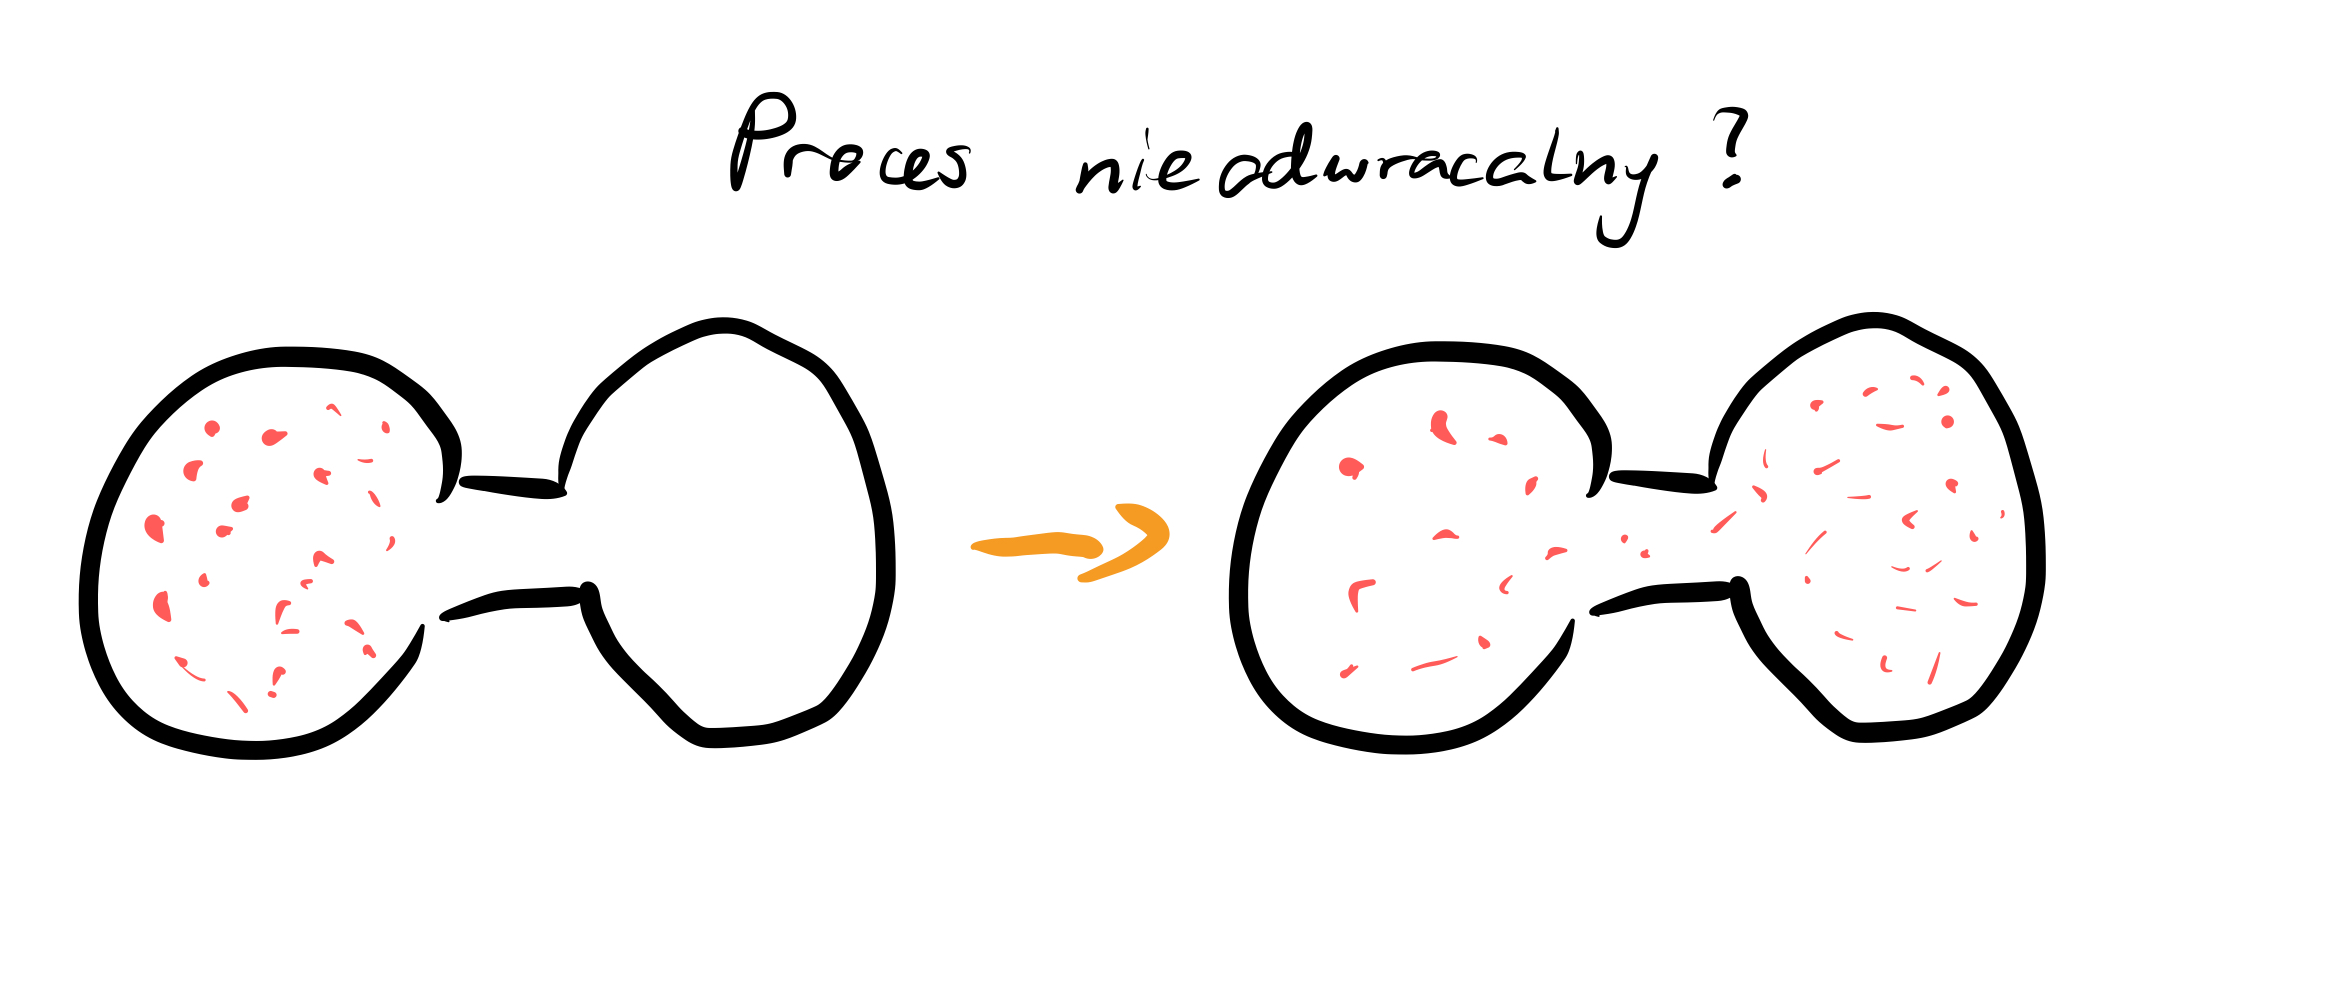
\includegraphics[width=0.8\linewidth]{Wyk_1_Rys_1.jpeg}
    \caption{Proces nieodwracalny?}
\end{figure}

\FloatBarrier

\subsection{Pokazy}
\subsubsection{Cylindry z ulepkiem cukru}
Widzimy tu na demonstracji \ind{odwracalność}. Są dwa rodzaje:
\begin{itemize}
    \item {\color{blue} odwracalność dynamiczna} \index{odwracalność!dynamiczna}:
    \[m \dv{v}{t} = F\]
    Wynika ona z dynamiki Newtonowskiej, jest symetryczna względem transformacji $t \to -t$, $v \to -v$.
    \item {\color{blue} odwracalność kinematyczna} \index{odwracalność!kinematyczna}:
    \[0 = m \dv{v}{t} = F - \gamma v \implies v = \frac{F}{\gamma}\]
    Jest symetryczna względem przekształcenia $F \to -F, v \to -v$. Ten rodzaj odwracalności zachodzi w lepkich cieczach. Symetryczny względem zmiany kierunku siły i prędkości, ale z czasem nieodwracalnym.
\end{itemize}

\begin{figure}[h!]
    \centering
    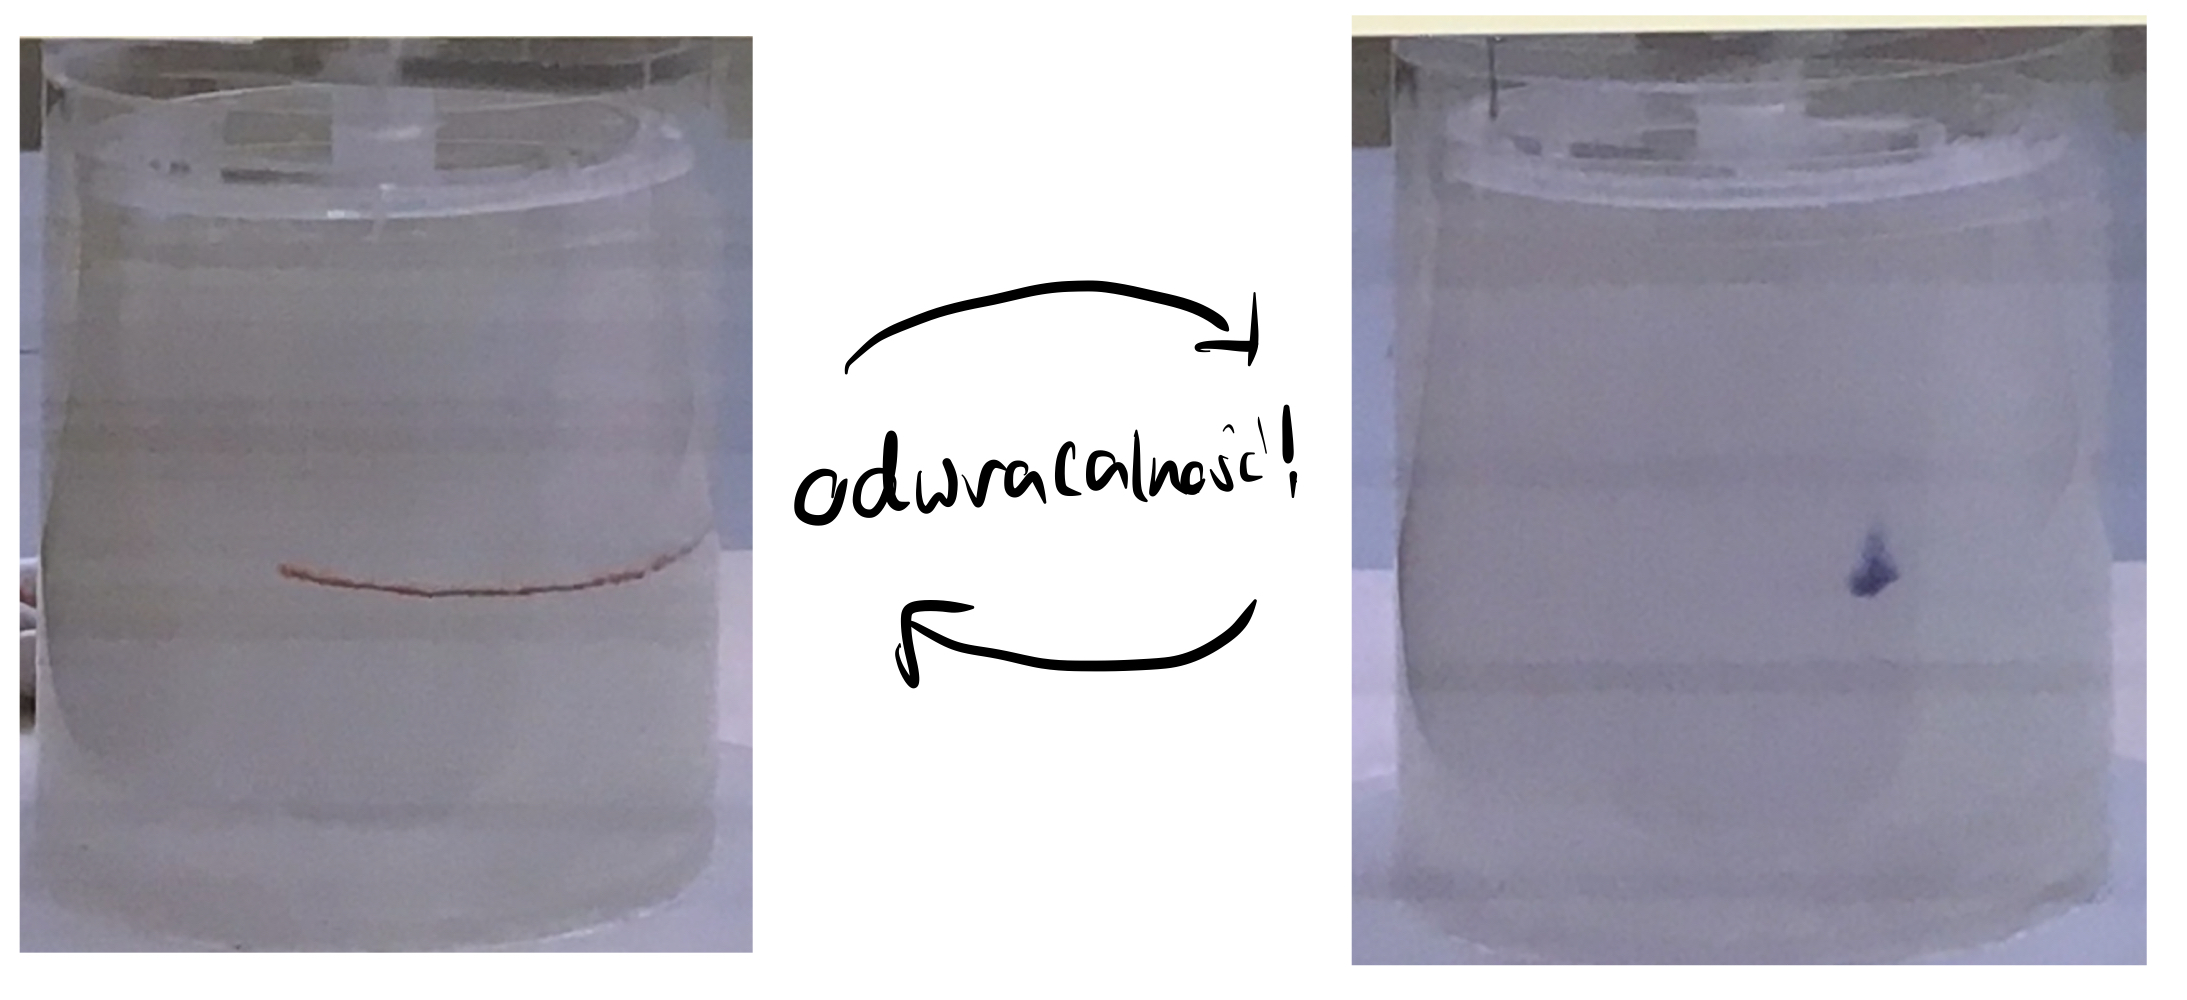
\includegraphics[width=0.8\linewidth]{Wyk_1_Rys_2.jpeg}
    \caption{Demonstracja odwracalności kinematycznej. Działa to tylko dla \emph{lepkiej cieczy}.}
\end{figure}

Kolejnym pojęciem które się pojawia jest \ind{ergodyczność}. Oznacza to, że średnia $\expval{x}$ z układu  po czasie jest równa średniej po powierzchni. Przykładem takiego układu jest zasadniczo \emph{Bilard bunimowicza} \ref{fig:bilard_bunimowicza}. Układ ergodyczny to taki, który po odpowiednio dużym czasie osiąga stan równowagi.

\begin{figure}[h!]
    \centering
    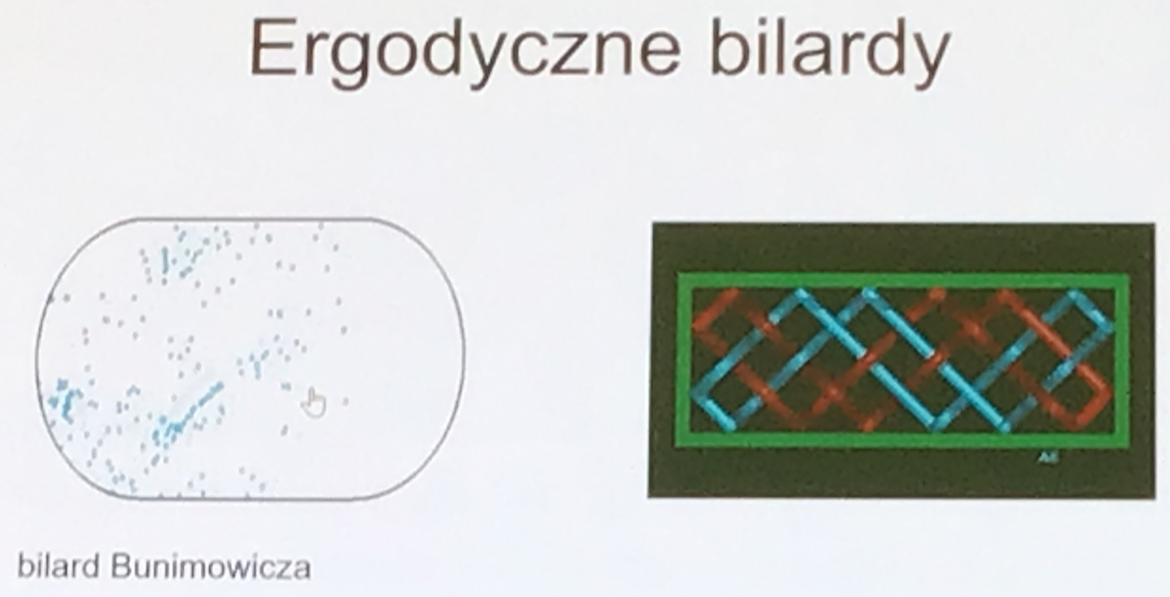
\includegraphics[width=0.8\linewidth]{Wyk_1_Rys_3.jpeg}
    \label{fig:bilard_bunimowicza}
    \caption{Demonstracja \emph{Bilardu Bunimowicza}. Po prawej bilard prostokątny - NieErgodyczny, ponieważ po odpowiednio długim czasie nie uśrednia się rozkład cząstek - Nie osiąga równowagi.}
\end{figure}

\emph{Model Ehrenfestów}:
\begin{figure}[h!]
    \centering
    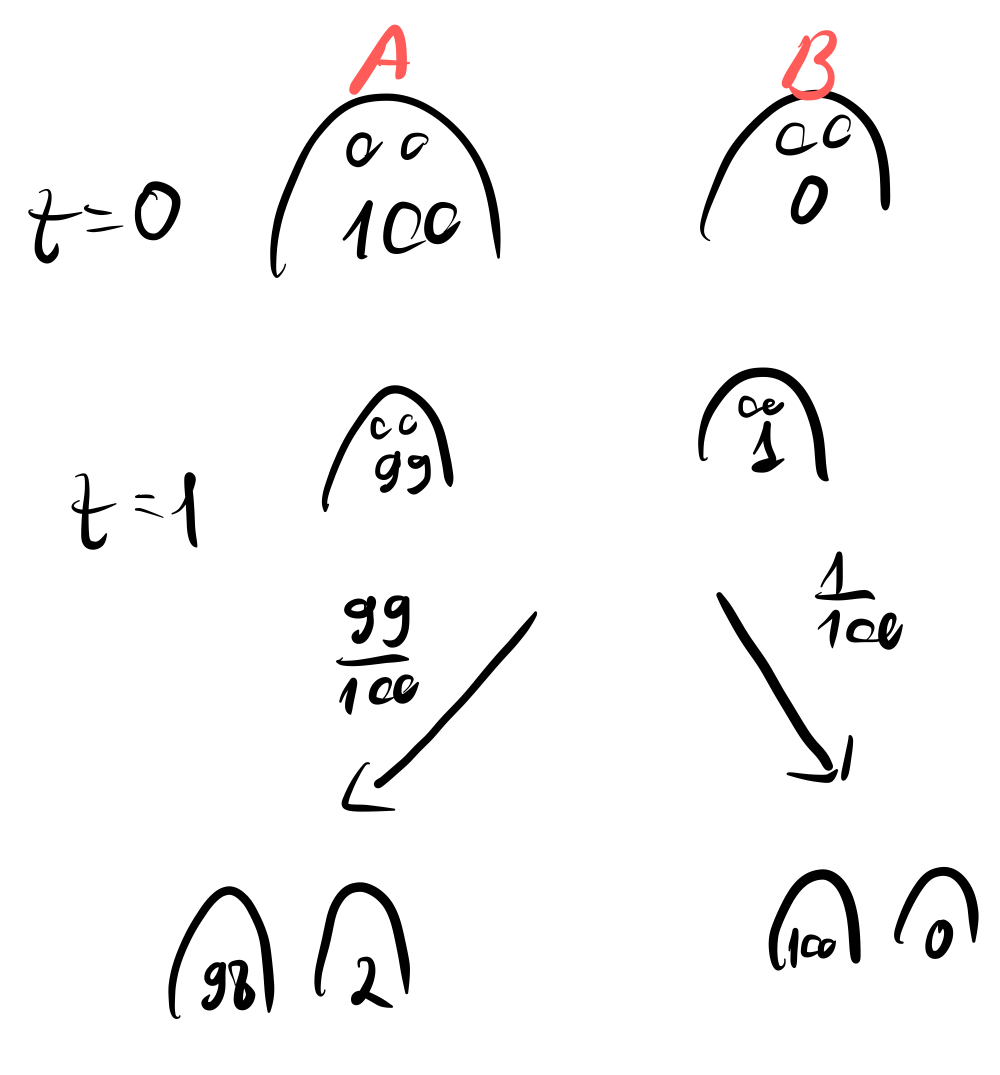
\includegraphics[width=0.8\linewidth]{Wyk_1_Rys_4.jpeg}
    \caption{Demonstracja \emph{Modelu Ehrenfestów}. Bierzemy dwa psy i liczymy sobie $\expval{n_a(t)}$. W tym celu patrzymy sobie na \ind{ansambl} (zespół) dwójek psów.}
    \label{fig:pchły}
\end{figure}

\printindex

\end{document}